\documentclass{exam}

\usepackage{units} 
\usepackage{xfrac} 
\usepackage[fleqn]{amsmath}
\usepackage{cancel}
\usepackage{float}
\usepackage{mdwlist}
\usepackage{booktabs}
\usepackage{cancel}
\usepackage{polynom}
\usepackage{caption}
\usepackage{fullpage}
\usepackage{comment}
\usepackage{enumerate}
\usepackage{graphicx}

\newcommand{\degree}{\ensuremath{^\circ}} 
\everymath{\displaystyle}

\printanswers

\ifprintanswers 
  \usepackage{2in1, lscape} 
\fi

\author{}
\date{\today}
\title{Statistics \\ Homework Three}

\begin{document}

  \maketitle

  \ifprintanswers
  \else
    \begin{itemize*}
      \item read Chapter 3 
      \item answer the questions in ``Check Your Skills'' and check the answers in the back of the book
      \item hand in exercises 25-27, 29-30, 32, 37-39, 41-44, 50-51
    \end{itemize*}
  \fi

  \ifprintanswers
    \begin{description}
      \item[26] 95\% of the people will be within two standard deviations of the mean.  

        mildly obese:
        \begin{align*}
          x_{min} &= 373 - 67 * 2 = 239 \\
          x_{max} &= 373 + 67 * 2 = 507 \\
        \end{align*}

        95\% of the mildly obese people will have between 239 and 507 minutes of activity per day.

        lean:
        \begin{align*}
          x_{min} &= 526 - 107 * 2 = 312 \\
          x_{min} &= 526 + 107 * 2 = 740 \\
        \end{align*}

        95\% of the lean people will have between 312 and 740 minutes of activity per day.

      \item[27]
        70 is two standard deviations below the mean.  Since 5\% of the people are more than two standard deviations
        from the mean and half of these are on the bottom end of the range, about 2.5\% will qualify. 

      \item[28]

        \begin{figure}[H]
          \centering
          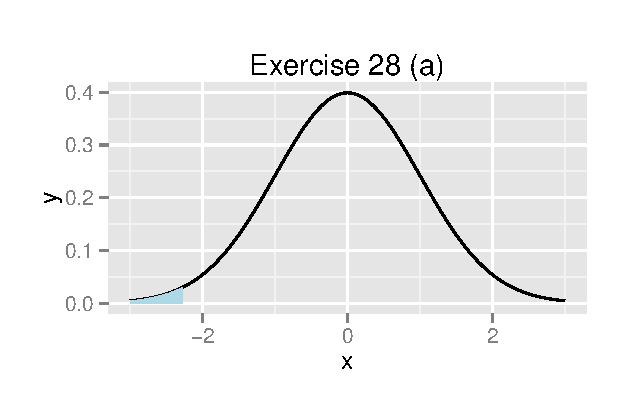
\includegraphics{figures/ex28a.eps}
          \caption{Exercise 28 (a)}
        \end{figure}

        \begin{figure}[H]
          \centering
          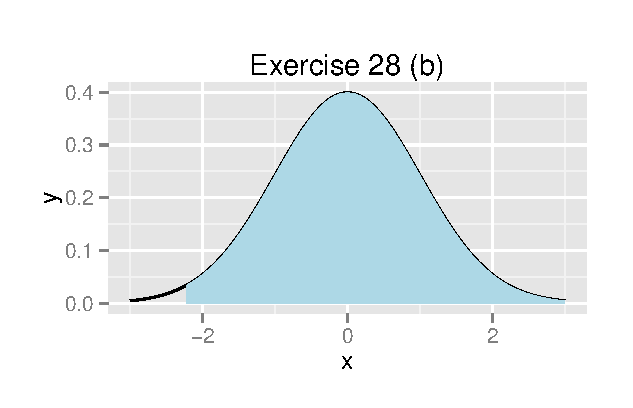
\includegraphics{figures/ex28b.eps}
          \caption{Exercise 28 (b)}
        \end{figure}

        \begin{figure}[H]
          \centering
          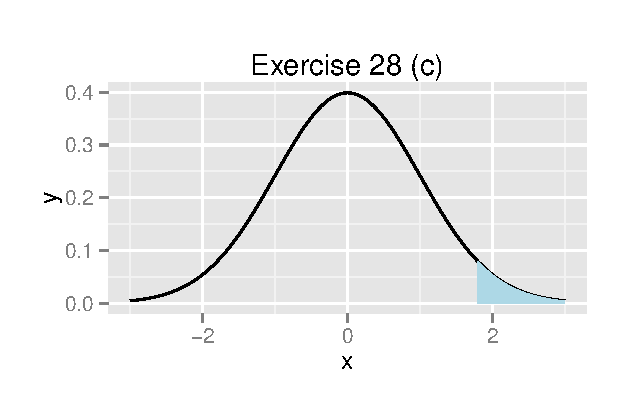
\includegraphics{figures/ex28c.eps}
          \caption{Exercise 28 (c)}
        \end{figure}

        \begin{figure}[H]
          \centering
          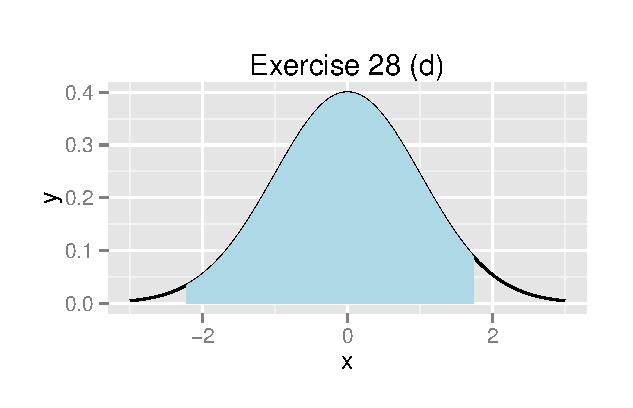
\includegraphics{figures/ex28d.eps}
          \caption{Exercise 28 (d)}
        \end{figure}

      \item[29]
        \begin{parts}
          \part $z = 0.84$
          \part $z = 0.39$ 
        \end{parts}

      \item[30]
        Standardize:
        \[
          z = \frac{5 - 7.11}{0.74} = -2.8513
        \]

        Use table A: 
        \[
          proportion = 0.0022 
        \]

      \item[31]
        Standardize:
        \[
          z = \frac{5 - 5.4}{0.54} = -0.7407407
        \]

        Use table A: 
        \[
          proportion = 0.2296 
        \]

      \item[32]
        \begin{parts}
          \part 
            Standardize:
            \[
              z = \frac{130 - 104}{12.5} = 2.08
            \]

            Use table A to find the percentage with heart rates below 130: 
            \[
              p_{below} = 98.12 \%
            \]

            Subtract from 100\% to find the percentage with heart rates above 130:
            \[
              p_{above} = \boxed{ 1.876 \% }
            \]

          \part 
            For the non-runners, 130 is the mean, so 50\% of the non-runners are above 130.

        \end{parts}

      \item[33]
        Standardize:
        \begin{align*}
          z_{min} & = \frac{0.8720 - 0.8750}{0.0012} = -2.5 \\
          z_{max} & = \frac{0.8780 - 0.8750}{0.0012} = 2.5 \\
        \end{align*}

        Use table A to find the proportions below the min/max
        \begin{align*}
          p_{min} & = 0.006210 \\
          p_{max} & = 0.9938 \\
        \end{align*}

        Subtract to find the proportion that meet the specifications:
        \[
          p_{good} = 0.9938 - 0.00621 = \boxed{ 0.9876 }
        \]

      \item[34]
        \begin{parts}
          
          \part
            Standardize:
            \begin{align*}
              z_{min} &= \frac{11.2 - 11.5}{0.2} = -1.5 \\
              z_{max} &= \frac{12.2 - 11.5}{0.2} = 3.5 \\
            \end{align*}

            Use table A to find the proportions below the min/max
            \begin{align*}
              p_{min} & = 0.0668 \\
              p_{max} & = 0.9998 \\
            \end{align*}

            Subtract to find the proportion that meet the specifications:
            \[
              p_{good} = 0.9998 - 0.0668 = \boxed{ 0.9330 }
            \]

            \part
              Standardize:
              \begin{align*}
                z_{min} &= \frac{11.2 - 11.7}{0.2} = -2.5 \\
                z_{max} &= \frac{12.2 - 11.7}{0.2} = 2.5 \\
              \end{align*}

              Use table A to find the proportions below the min/max
              \begin{align*}
                p_{min} & = 0.0062 \\
                p_{max} & = 0.9938 \\
              \end{align*}

              Subtract to find the proportion that meet the specifications:
              \[
                p_{good} = 0.9938 - 0.0062 = \boxed{ 0.9876 }
              \]

        \end{parts}

      \item[35]
        Standardize:
        \[
          z = \frac{25 - 18.7}{4.3} = 1.4651 \\
        \]

        Use table A: 
        \[
          p = 92.86 \% \\
        \]

      \item[35]
        Use table A to find how many standard deviations above the mean 90\% is: 
        \[
          z = \unit[1.2816]{sd}
        \]

        Convert to MPG
        \[
          x = 18.7 + 1.2816 \cdot 4.3 = \unit[24.21]{MPG}
        \]

    \end{description}

  \else
    \vspace{11 cm}
    \begin{quote}
      \begin{em}
        Even voting for the right is doing nothing for it. It is only expressing to men feebly your desire that it
        should prevail. 
        % A wise man will not leave the right to the mercy of chance, nor wish it to prevail through the power of the
        % majority. There is but little virtue in the action of masses of men. When the majority shall at length vote for
        % the abolition of slavery, it will be because they are indifferent to slavery, or because there is but little
        % slavery left to be abolished by their vote. 
      \end{em}
    \end{quote}
    \hspace{1 cm} --Henry David Thoreau
  \fi

\end{document}

